\section{Materiales y métodos}

En esta sección, describiremos la metodología utilizada en el estudio de la Disgrafia,
junto con los materiales empleados. La metodología se dividió en varias etapas, las
cuales se detallarán a lo largo de esta sección y se pueden observar en la imagen \ref{fig:workflow}.

\begin{figure}[h!]
	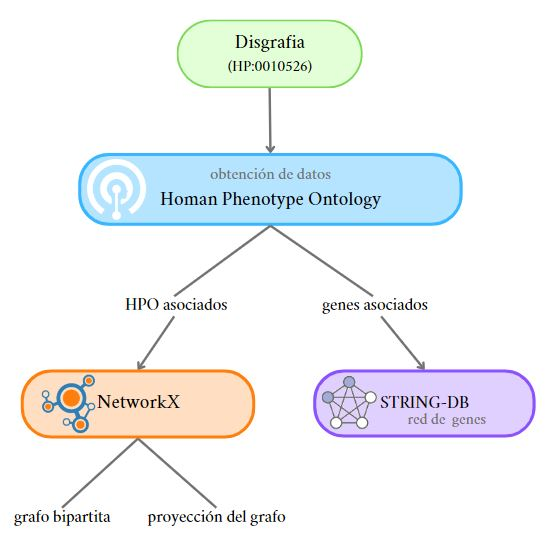
\includegraphics[width=0.9\textwidth]{figures/workflow.JPG}
	\caption{Flujo de trabajo}
	\label{fig:workflow}
\end{figure}

El fenotipo de estudio es la Disgrafía. Lo primero que se realizó fue buscar este fenotipo en la Human Phenotype Ontology \cite{HPO2021}, conociendo que su identificador es HP:0010526. De esta base de datos, obtuvimos un archivo tabulado que enumera para cada gen las clases HPO más específicas. Las primeras cinco filas se pueden visualizar en la tabla \ref{tabla:geneshpo}.

\begin{table}[h]
	\centering
	\caption{Cabecera del archivo}
	\label{tabla:geneshpo}
	\resizebox{1.1\textwidth}{!}{
		\begin{tabular}{|c|c|c|c|c|c|c|}
			\hline
			Gene id (ncbi) & Gene symbol & HPO id & HPO name & frequency & Disease id \\
			\hline
			10 & NAT2 & HP:0000007 & Autosomal recessive inheritance & - & OMIM:243400 \\
			10 & NAT2 & HP:0001939 & Abnormality of metabolism/homeostasis & - & OMIM:243400 \\
			16 & AARS1 & HP:0002460 & Distal muscle weakness & 15/15 & OMIM:613287 \\
			16 & AARS1 & HP:0002451 & Limb dystonia & 3/3 & OMIM:616339 \\
			16 & AARS1 & HP:0008619 & Bilateral sensorineural hearing impairment & HP:0040283 & ORPHA:33364 \\
			\hline
		\end{tabular}
	}
\end{table}

La tabla \ref{tabla:geneshpo} proporciona el identificador de gen NCBI, el símbolo del gen, el identificador HPO y el nombre del término. Si está disponible, se muestra la frecuencia. Por ejemplo, la mutación en el gen AARS1 causa \textit{leucoencefalopatía}. La frecuencia del término HPO Ataxia sensorial esta anotada como 1 de 2 debido a la información en Sundal C, et al. \cite{Sundal2019}. La última columna muestra anotaciones realizadas por el equipo HPO (utilizando identificadores de enfermedades de OMIM), así como anotaciones proporcionadas por el equipo de Orphanet (utilizando identificadores de enfermedades de ORPHA).